\paragraph{Activity Diagrams}
Activity diagrams illustrate the dynamic behavior of the system by modeling workflows, decision points, and parallel activities involved in the AI-Enhanced Online Assessment and Monitoring System. These diagrams provide a clear, step-by-step representation of how different users interact with the system and how the system responds to various conditions. Activity diagrams are particularly effective in representing complex processes such as online examinations, AI-based proctoring, automated grading, and administrative decision-making, where conditional logic and exception handling are essential.

The system’s activity diagrams are organized into four main workflows:

\begin{enumerate}
    \item \textbf{Enterprise Registration \& Authentication:} This activity diagram illustrates the process through which an enterprise registers and gains access to the system. The workflow begins when an organization submits its registration details. The system then forwards the request for administrative approval. A decision node determines whether the registration is approved or rejected. If approved, the enterprise selects a subscription plan and completes payment before accessing the system dashboard. If the payment fails or the registration is rejected, the system notifies the enterprise accordingly and terminates the process. This workflow ensures controlled system access and subscription enforcement.
    \vspace*{0.5em}
    \begin{figure}[H]
    \centering
    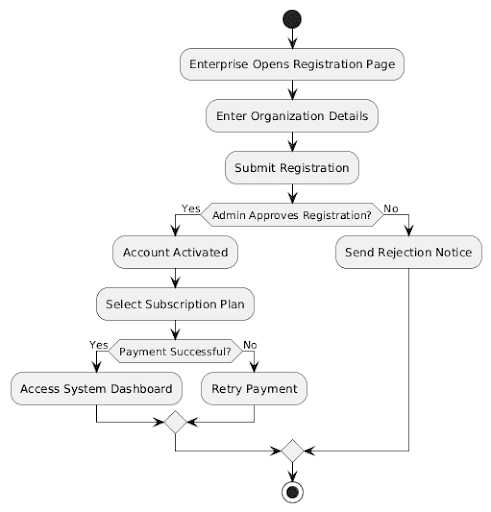
\includegraphics[width=1\linewidth,keepaspectratio]{assets/activity_diagrams/Enterprise Registration and Authentication.png}
    \caption{Enterprise Registration and Authentication Activity Diagram}
    \label{fig:enterprise-registration-authentication}
    \end{figure}

    \item \textbf{Exam Creation \& Scheduling:} This activity diagram represents the steps followed by an administrator to create and schedule an examination. The process starts with the administrator logging into the system and opening the exam creation module. The administrator configures exam parameters such as question types, duration, passing score, and randomization rules. A decision point determines whether candidates are added immediately or the exam is saved as a draft. Once candidates are assigned and the schedule is confirmed, the exam is published. This workflow supports flexibility while maintaining structured exam configuration.
    \vspace*{0.5em}
    \begin{figure}[H]
    \centering
    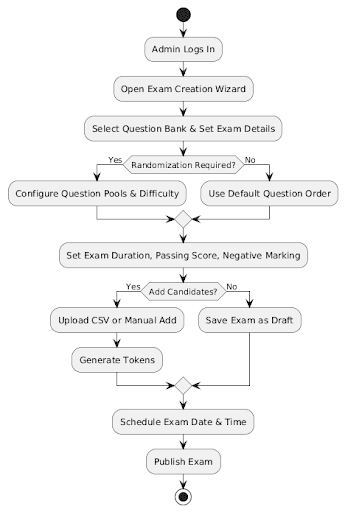
\includegraphics[width=0.8\linewidth,keepaspectratio]{assets/activity_diagrams/Exam Creation and Scheduling.png}
    \caption{Exam Creation and Scheduling Activity Diagram}
    \label{fig:exam-creation-scheduling}
    \end{figure}

    \item \textbf{Candidate Exam + AI Proctoring:} This activity diagram describes the flow of events when a candidate takes an examination. The process begins when the candidate logs in using a secure token or credentials. The system performs identity verification using facial recognition before allowing exam access. During the exam, AI-based proctoring continuously monitors candidate behavior. A decision node evaluates whether suspicious behavior is detected. If a violation occurs, the system logs the event and may terminate the exam depending on severity. Otherwise, the candidate continues until submission or time expiration. This workflow emphasizes exam integrity and real-time monitoring.
    \vspace*{0.5em}
    \begin{figure}[H]
    \centering
    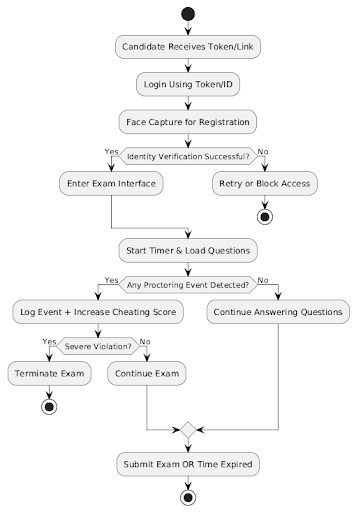
\includegraphics[width=.75\linewidth,keepaspectratio]{assets/activity_diagrams/Candidate Exam and AI Proctoring.png}
    \caption{Candidate Exam and AI Proctoring Activity Diagram}
    \label{fig:candidate-exam-ai-proctoring}
    \end{figure}

    \item \textbf{Grading + Certificate Generation:} This activity diagram illustrates the post-exam evaluation process. It begins when an exam submission is received by the system. Objective questions are graded automatically, while subjective answers, if present, are forwarded for manual blind grading. The system then calculates the final score and analyzes proctoring logs to determine cheating probability. A decision point checks whether the candidate meets both academic and integrity requirements. Successful candidates receive a digital certificate, while unsuccessful or suspicious cases are flagged for review. This workflow ensures fair assessment and result transparency.
    \vspace*{0.5em}
    \begin{figure}[H]
    \centering
    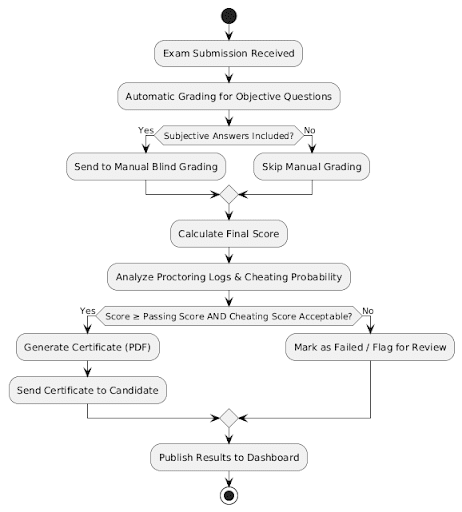
\includegraphics[width=0.8\linewidth,keepaspectratio]{assets/activity_diagrams/Grading and Certificate Generation.png}
    \caption{Grading and Certificate Generation Activity Diagram}
    \label{fig:grading-certificate-generation}
    \end{figure}
\end{enumerate}
